\documentclass[11pt, oneside]{article}   	% use "amsart" instead of "article" for AMSLaTeX format
\usepackage{geometry}                		% See geometry.pdf to learn the layout options. There are lots.
\geometry{letterpaper}                   		% ... or a4paper or a5paper or ... 
%\geometry{landscape}                		% Activate for rotated page geometry
%\usepackage[parfill]{parskip}    		% Activate to begin paragraphs with an empty line rather than an indent
\usepackage{graphicx}				% Use pdf, png, jpg, or eps§ with pdflatex; use eps in DVI mode
								% TeX will automatically convert eps --> pdf in pdflatex		
\usepackage{amssymb}
\usepackage{amsmath}
\usepackage{enumitem}
\usepackage{caption}
\usepackage{subcaption}
\usepackage{multirow}
\usepackage{array}
\usepackage{float}
\usepackage{natbib}
%\usepackage{enumitem}

%SetFont

%SetFonts


\title{Project \#4}
\author{Huiyu Wang\\604--592--364}
\date{}							% Activate to display a given date or no date

\begin{document}
\maketitle

\section{bark}
\begin{figure}[H]
	\centering
	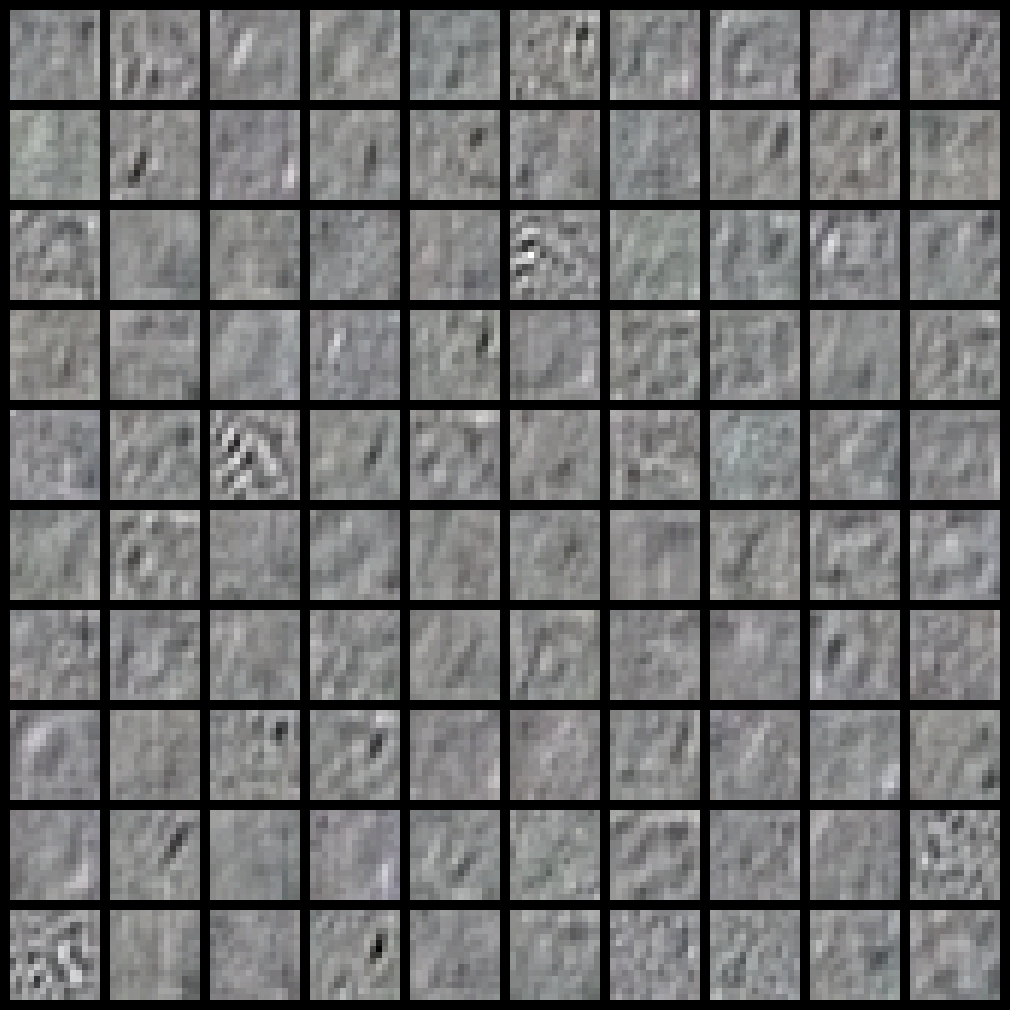
\includegraphics[width=0.8\textwidth]{bark}
	\caption{Normalized filters in the first layer}
	\label {fig:barkf}
\end{figure}

\begin{figure}[H]
    \centering
    \begin{subfigure}[b]{0.45\textwidth}
        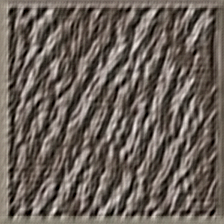
\includegraphics[width=\textwidth]{figure/bark/layer_01_001}
        \caption{layer 1 synthesis}
    \end{subfigure}
    \begin{subfigure}[b]{0.45\textwidth}
        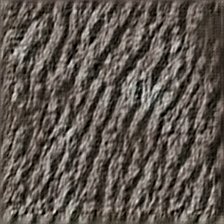
\includegraphics[width=\textwidth]{figure/bark/layer_02_001}
        \caption{layer 2 synthesis}
    \end{subfigure}
    
    \begin{subfigure}[b]{0.45\textwidth}
        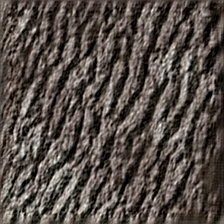
\includegraphics[width=\textwidth]{figure/bark/layer_03_001}
        \caption{layer 3 synthesis}
    \end{subfigure}
        \begin{subfigure}[b]{0.45\textwidth}
        
\includegraphics[width=\textwidth]{figure/bark/layer_00_001}
        \caption{original image}
    \end{subfigure}
    \caption{Synthesized Images (bark)}\label{fig:barks}
\end{figure}

\section{beehive}
\begin{figure}[H]
	\centering
	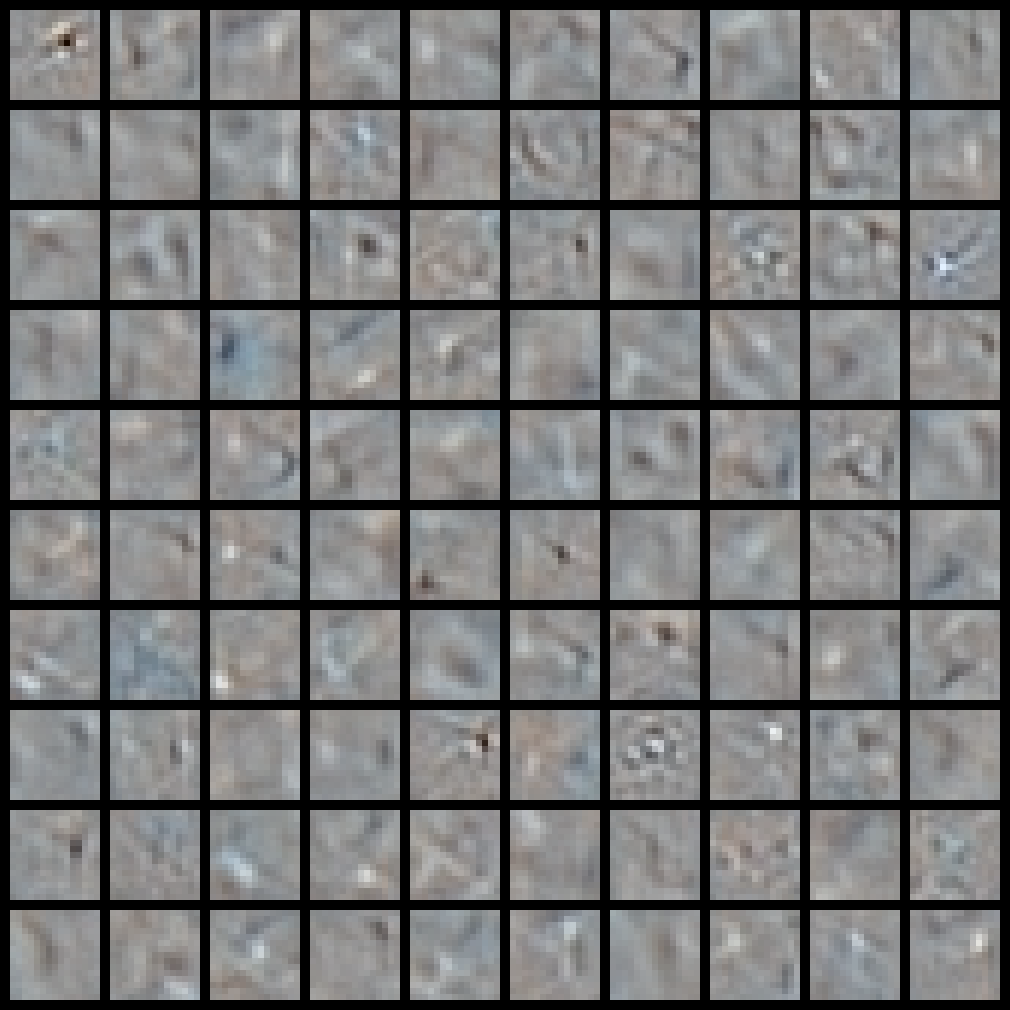
\includegraphics[width=0.8\textwidth]{beehive}
	\caption{Normalized filters in the first layer}
	\label {fig:beehivef}
\end{figure}

\begin{figure}[H]
    \centering
    \begin{subfigure}[b]{0.45\textwidth}
        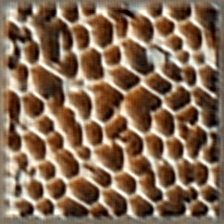
\includegraphics[width=\textwidth]{figure/beehive/layer_01_001}
        \caption{layer 1 synthesis}
    \end{subfigure}
    \begin{subfigure}[b]{0.45\textwidth}
        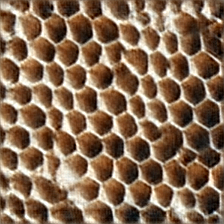
\includegraphics[width=\textwidth]{figure/beehive/layer_02_001}
        \caption{layer 2 synthesis}
    \end{subfigure}
    
    \begin{subfigure}[b]{0.45\textwidth}
        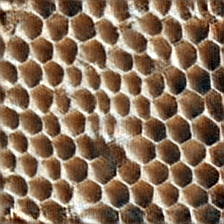
\includegraphics[width=\textwidth]{figure/beehive/layer_03_001}
        \caption{layer 3 synthesis}
    \end{subfigure}
        \begin{subfigure}[b]{0.45\textwidth}
        
\includegraphics[width=\textwidth]{figure/beehive/layer_00_001}
        \caption{original image}
    \end{subfigure}
    \caption{Synthesized Images (beehive)}\label{fig:beehives}
\end{figure}

\section{coffee}
\begin{figure}[H]
	\centering
	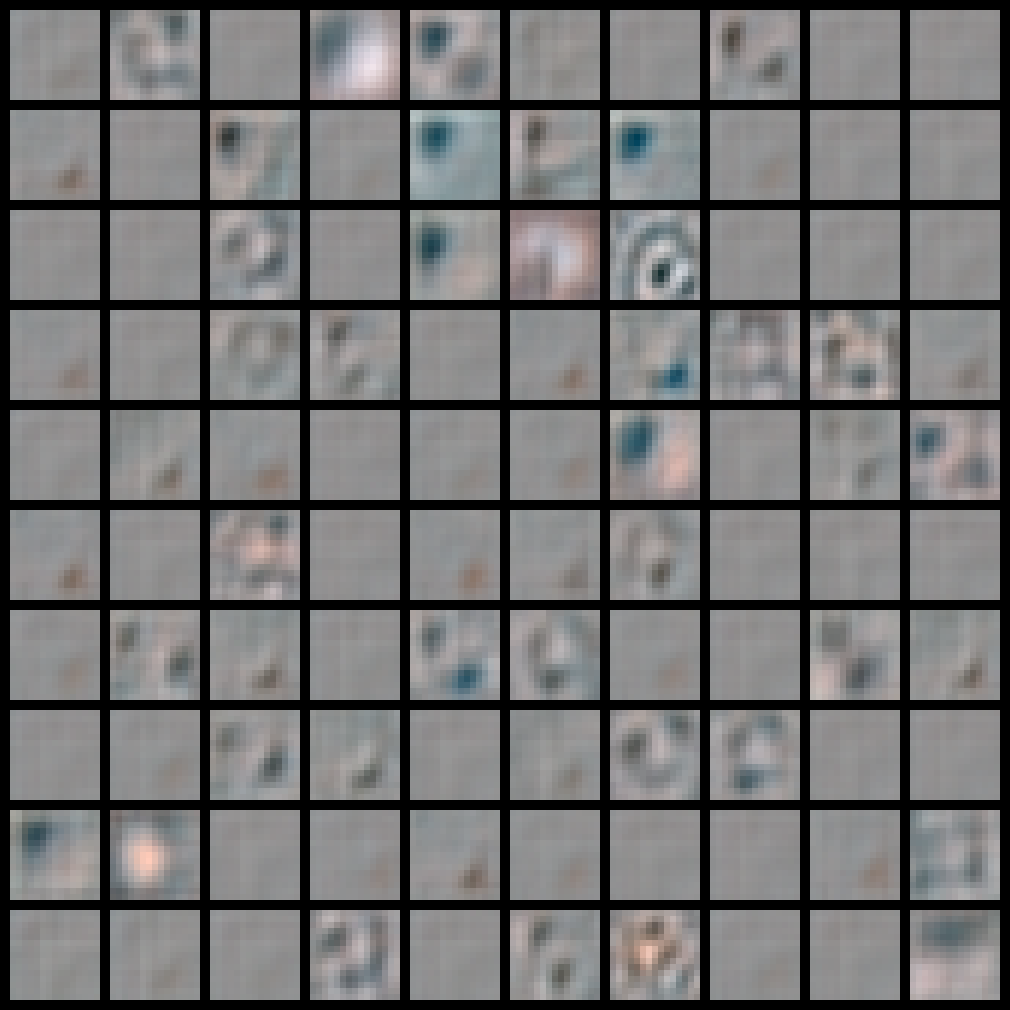
\includegraphics[width=0.8\textwidth]{coffee}
	\caption{Normalized filters in the first layer}
	\label {fig:coffeef}
\end{figure}

\begin{figure}[H]
    \centering
    \begin{subfigure}[b]{0.45\textwidth}
        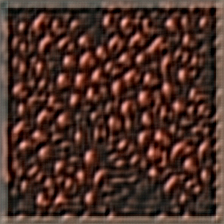
\includegraphics[width=\textwidth]{figure/coffee/layer_01_001}
        \caption{layer 1 synthesis}
    \end{subfigure}
    \begin{subfigure}[b]{0.45\textwidth}
        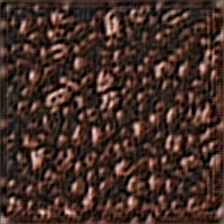
\includegraphics[width=\textwidth]{figure/coffee/layer_02_001}
        \caption{layer 2 synthesis}
    \end{subfigure}
    
    \begin{subfigure}[b]{0.45\textwidth}
        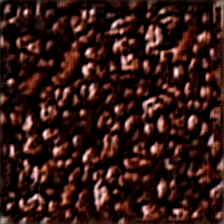
\includegraphics[width=\textwidth]{figure/coffee/layer_03_001}
        \caption{layer 3 synthesis}
    \end{subfigure}
        \begin{subfigure}[b]{0.45\textwidth}
        
\includegraphics[width=\textwidth]{figure/coffee/layer_00_001}
        \caption{original image}
    \end{subfigure}
    \caption{Synthesized Images (coffee)}\label{fig:coffees}
\end{figure}

\section{rose}
\begin{figure}[H]
	\centering
	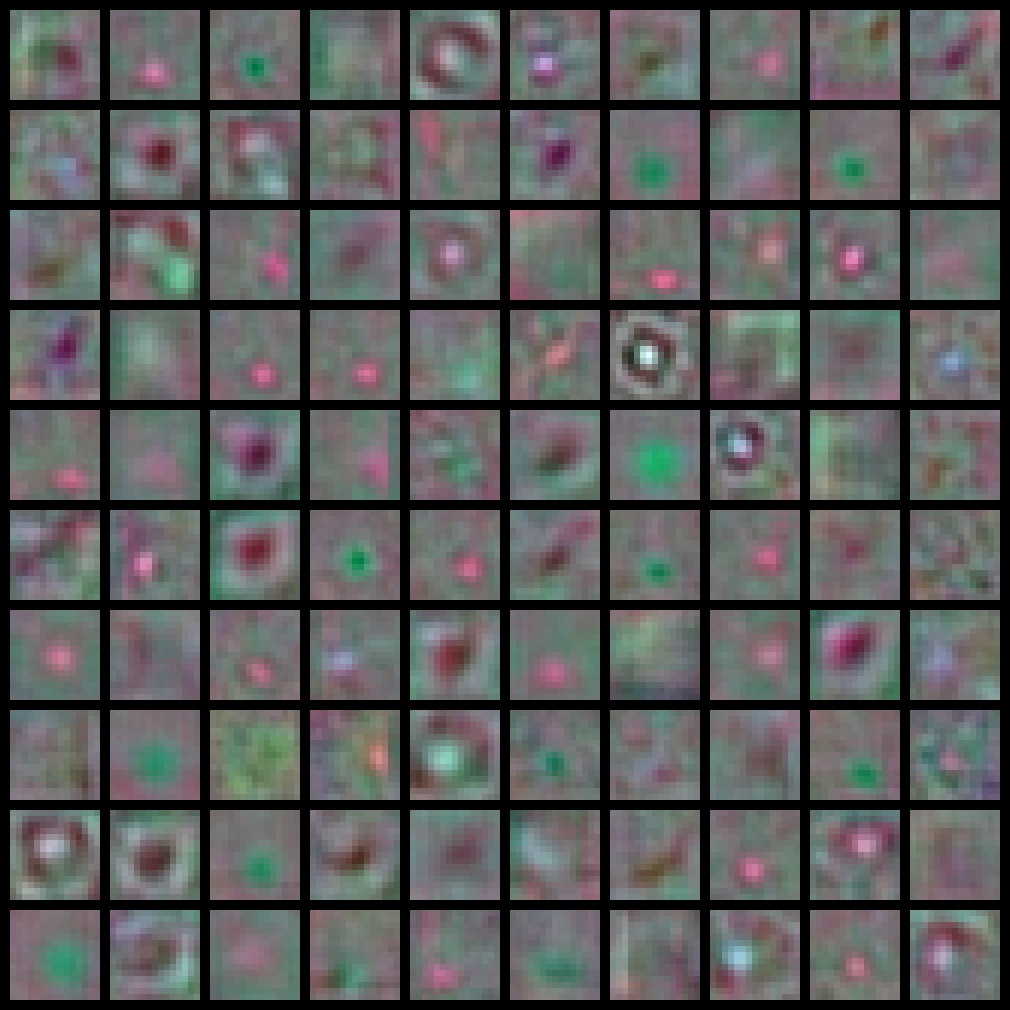
\includegraphics[width=0.8\textwidth]{rose}
	\caption{Normalized filters in the first layer}
	\label {fig:rosef}
\end{figure}

\begin{figure}[H]
    \centering
    \begin{subfigure}[b]{0.45\textwidth}
        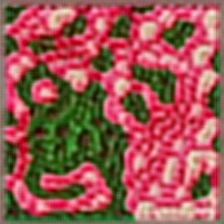
\includegraphics[width=\textwidth]{figure/rose/layer_01_001}
        \caption{layer 1 synthesis}
    \end{subfigure}
    \begin{subfigure}[b]{0.45\textwidth}
        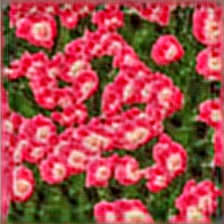
\includegraphics[width=\textwidth]{figure/rose/layer_02_001}
        \caption{layer 2 synthesis}
    \end{subfigure}
    
    \begin{subfigure}[b]{0.45\textwidth}
        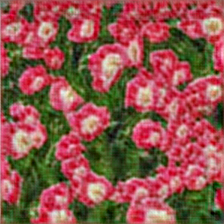
\includegraphics[width=\textwidth]{figure/rose/layer_03_001}
        \caption{layer 3 synthesis}
    \end{subfigure}
        \begin{subfigure}[b]{0.45\textwidth}
        
\includegraphics[width=\textwidth]{figure/rose/layer_00_001}
        \caption{original image}
    \end{subfigure}
    \caption{Synthesized Images (rose)}\label{fig:roses}
\end{figure}

\section{stucco}
\begin{figure}[H]
	\centering
	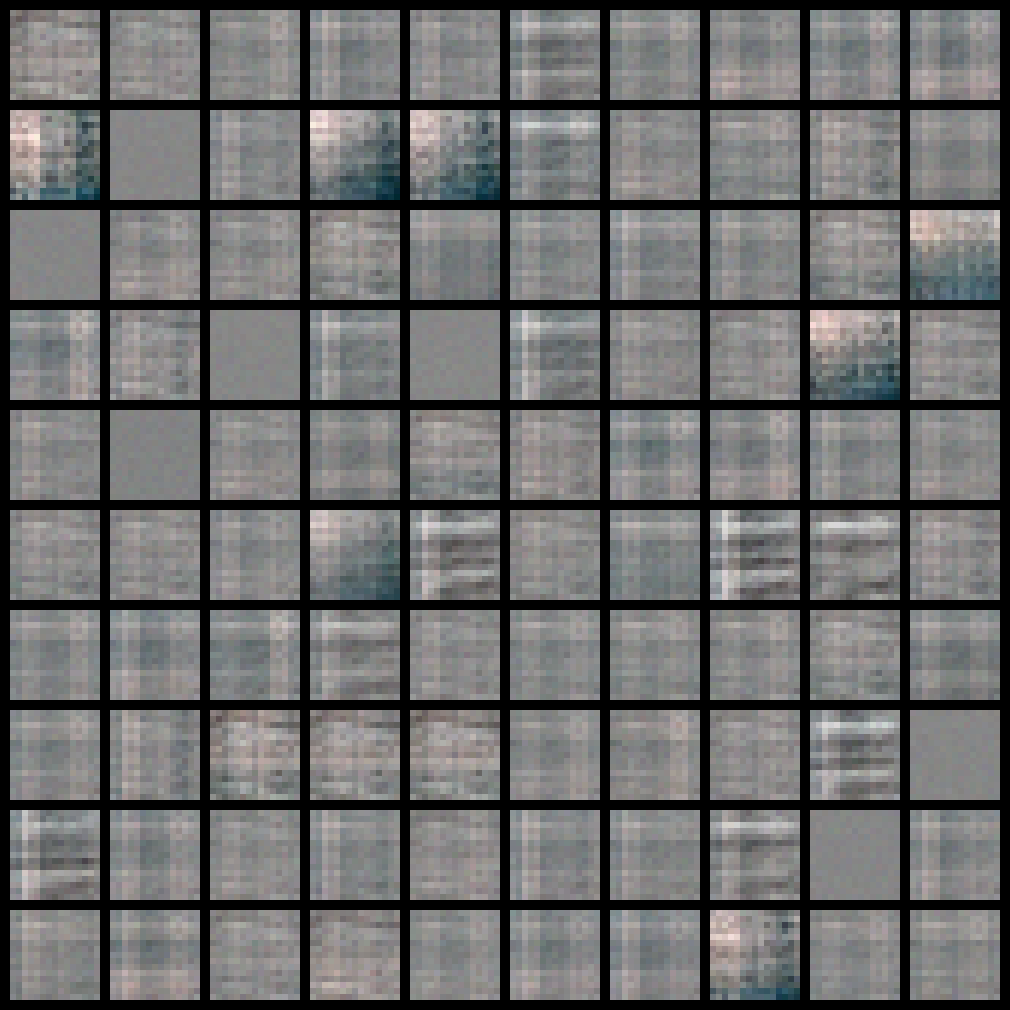
\includegraphics[width=0.8\textwidth]{stucco}
	\caption{Normalized filters in the first layer}
	\label {fig:stuccof}
\end{figure}

\begin{figure}[H]
    \centering
    \begin{subfigure}[b]{0.45\textwidth}
        
\includegraphics[width=\textwidth]{figure/stucco/layer_01_001}
        \caption{layer 1 synthesis}
    \end{subfigure}
    \begin{subfigure}[b]{0.45\textwidth}
        
\includegraphics[width=\textwidth]{figure/stucco/layer_02_001}
        \caption{layer 2 synthesis}
    \end{subfigure}
    
    \begin{subfigure}[b]{0.45\textwidth}
        
\includegraphics[width=\textwidth]{figure/stucco/layer_03_001}
        \caption{layer 3 synthesis}
    \end{subfigure}
        \begin{subfigure}[b]{0.45\textwidth}
        
\includegraphics[width=\textwidth]{figure/stucco/layer_00_001}
        \caption{original image}
    \end{subfigure}
    \caption{Synthesized Images (stucco)}\label{fig:stuccos}
\end{figure}

\section{water}
\begin{figure}[H]
	\centering
	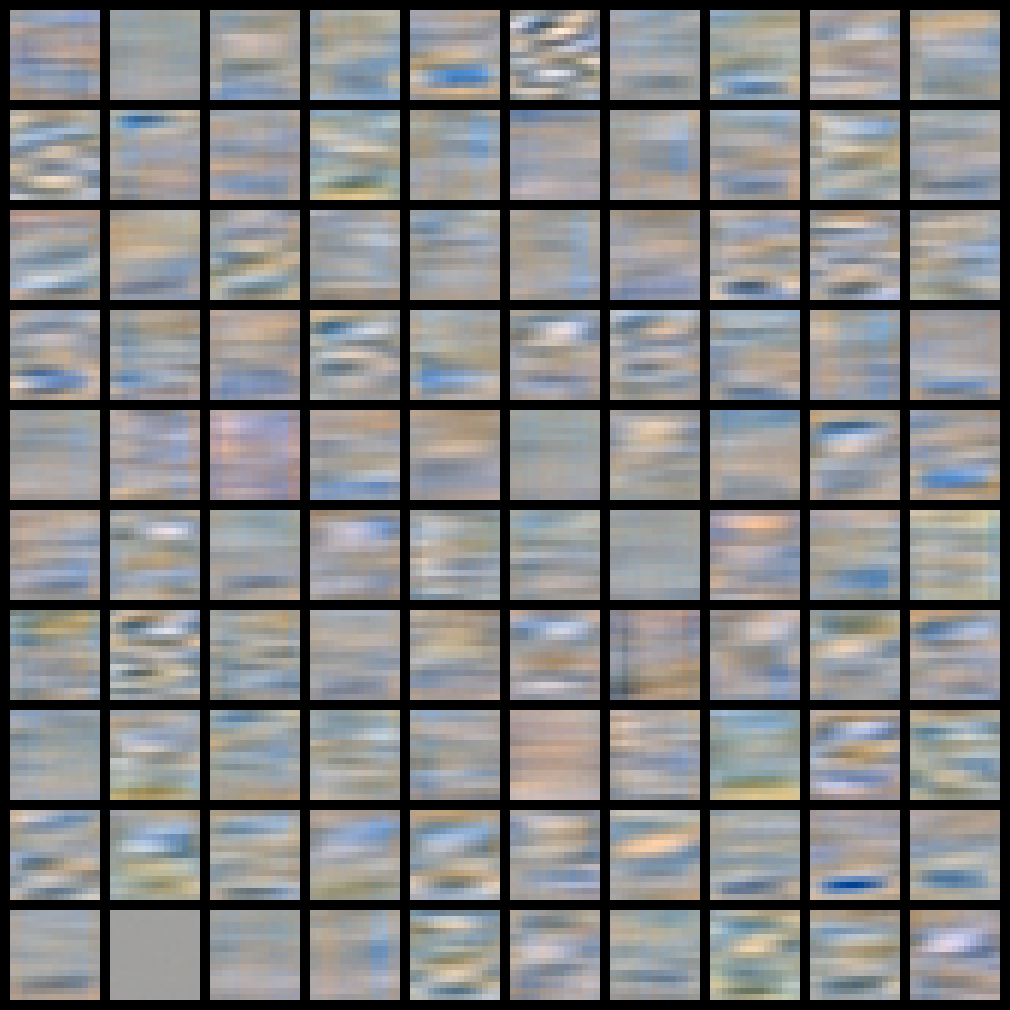
\includegraphics[width=0.8\textwidth]{water}
	\caption{Normalized filters in the first layer}
	\label {fig:waterf}
\end{figure}

\begin{figure}[H]
    \centering
    \begin{subfigure}[b]{0.45\textwidth}
        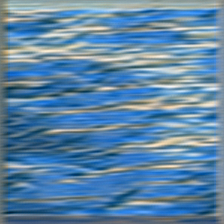
\includegraphics[width=\textwidth]{figure/water/layer_01_001}
        \caption{layer 1 synthesis}
    \end{subfigure}
    \begin{subfigure}[b]{0.45\textwidth}
        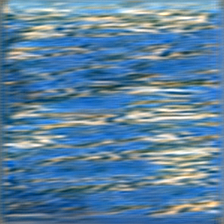
\includegraphics[width=\textwidth]{figure/water/layer_02_001}
        \caption{layer 2 synthesis}
    \end{subfigure}
    
    \begin{subfigure}[b]{0.45\textwidth}
        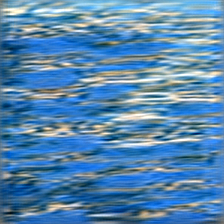
\includegraphics[width=\textwidth]{figure/water/layer_03_001}
        \caption{layer 3 synthesis}
    \end{subfigure}
        \begin{subfigure}[b]{0.45\textwidth}
        
\includegraphics[width=\textwidth]{figure/water/layer_00_001}
        \caption{original image}
    \end{subfigure}
    \caption{Synthesized Images (water)}\label{fig:waters}
\end{figure}

\section{conclusion}
After trying different parameters, such as one-layer-extra-large-filters, two-layer-default-setting, three-layer-$7\times7$-filters, five-layer-$3\times3$-filters, and different strides and number of filters. We find out the parameters used in \cite{xie2016theory} give the best synthesized results. The first layer has 100 $15\times15$ filters with stride = 3 and padding size = 2. The second layer has 64 $5\times5$ filters with stride = 1 and padding size = 2. The third layer has 30 $3\times3$ filters with stride = 1 and padding size = 2. Also the Langevin dynamics runs 20 steps for each sample. The normalized filters and the results are shown in Figure \ref{fig:barkf} - \ref{fig:waters}.

We can see that this model can fit the original image using the potential function of negative summation of total filtered response in the top layer, which will encourage the model to generate meaningful patterns. The synthesized images cannot be told apart from the original image if one is looking at the images from far away. However, the synthesized images don't have vivid details. They are like a little bit blurry especially when it comes to stucco, most of features of which are detailed textures rather than high level patterns. This may be because the first layer filters are too large to fit the local details or maybe we also need to put constraints to the filtered results like in project 3. Actually code in project 3 gives better result for stucco textures and details as shown in figure \ref{fig:3}.

\begin{figure}[H]
	\centering
	
\includegraphics[width=0.8\textwidth]{stucco4}
	\caption{Stucco synthesized using code in project 3}
	\label {fig:3}
\end{figure}

\bibliographystyle{plain}
\bibliography{xie2016theory}

\end{document}  